\documentclass[aspectratio=169]{beamer}
\usepackage{ulem}
\usepackage{tikz}
\usepackage{booktabs}
 \usepackage{graphicx,threeparttable,caption}
\usetikzlibrary{shapes,snakes}
\usepackage[beamer,customcolors]{hf-tikz}
\usepackage{nicematrix}
\usepackage{xcolor}
\usepackage{makecell}
\usepackage{array}
\usepackage{csquotes}
\usepackage{csquotes}
\usepackage{minted}
\captionsetup{labelformat=empty,labelsep=none}

\graphicspath{ {./png/} }

\usetikzlibrary{
    arrows,
    arrows.meta,
    shapes,
    positioning,
    shadows,
    trees,
    calc
}

\tikzset{%
    >={Latex[width=2mm,length=2mm]},
    % Specifications for style of nodes:
    plain/.style = {},
    base/.style = {
        plain,
        rectangle, rounded corners, draw=black,
        minimum width=1cm, minimum height=1cm,
        text centered, font=\sffamily\tiny\bfseries,
        fill=white, align=center
    },
    app/.style = {base, ellipse},
    data/.style = {base, fill=gray!30},
    action/.style = {base, circle, fill=red!30},
    note/.style = {app, fill=yellow},
    hl/.style={
    set fill color=red!80!black!40,
    set border color=red!80!black
    }
}


\AtBeginSection[]{
  \begin{frame}
  \vfill
  \centering
  \begin{beamercolorbox}[sep=8pt,center,shadow=true,rounded=true]{title}
    \usebeamerfont{title}\insertsectionhead\par%
  \end{beamercolorbox}
  \vfill
  \end{frame}
}
%\usecolortheme[orchid]{structure}
\usetheme[hideothersubsections]{PaloAlto}
\makeatletter
\patchcmd{\csq@bquote@i}{{#6}}{{\emph{#6}}}{}{}
\makeatother
%\usecolortheme{orchid}
%\usefonttheme{professionalfonts}
\newcommand{\soutthick}[1]{%
   \textcolor{red}{
   \renewcommand{\ULthickness}{1pt}%
      \sout{#1}%
   \renewcommand{\ULthickness}{.4pt}% Resetting to ulem default
   }
}
\newcommand{\centered}[1]{\begin{tabular}{l} #1 \end{tabular}}
\setbeamertemplate{section in toc}[square]
\setbeamertemplate{subsection in toc}[square]
\setbeamertemplate{secion in sidebar}[shaded]
\setbeamertemplate{items}[square]
\setbeamercovered{transparent} 

\title[]{Introduction to Computational Social Science}
\subtitle{Microtargeting -- discussion}
\author[]{Mikołaj Biesaga\\ \small{\color{blue}{\href{mailto:m.biesaga@uw.edu.pl}{m.biesaga@uw.edu.pl}}}}
\institute{
\includegraphics[width = 4 cm]{uw.png}}
\date{\today}
\begin{document}
\begin{frame}
   \titlepage
\end{frame}

\begin{frame}
    \frametitle{Psychological Targeting}
    \only<1,4, 7>{
        \begin{itemize}
            \item 2007 David Stillwell creates \href{https://sites.google.com/michalkosinski.com/mypersonality}{\textcolor{blue}{myPersonality}} Facebook App to share a personality questionnaire
            \item by 2012 6 million people completed personality questionnaire
            \item 40\% of participants gave the informed consent to share their Facebook data
            \item Private traits and attributes are predictable from digital records of human behavior (Kosinski, Stillwell, \& Graepel, 2013)
            \item<4,7> Psychological targeting as an effective approach to digital mass persuasion (Matz et al., 2017)
            \item<7> Discussion with Matz et al. (Eckles, Gordon, \& Johnson, 2018; Sharp, Danenberg, \& Bellman, 2018)
        \end{itemize}
    }
    \only<2>{
        \begin{figure}
            \centering
            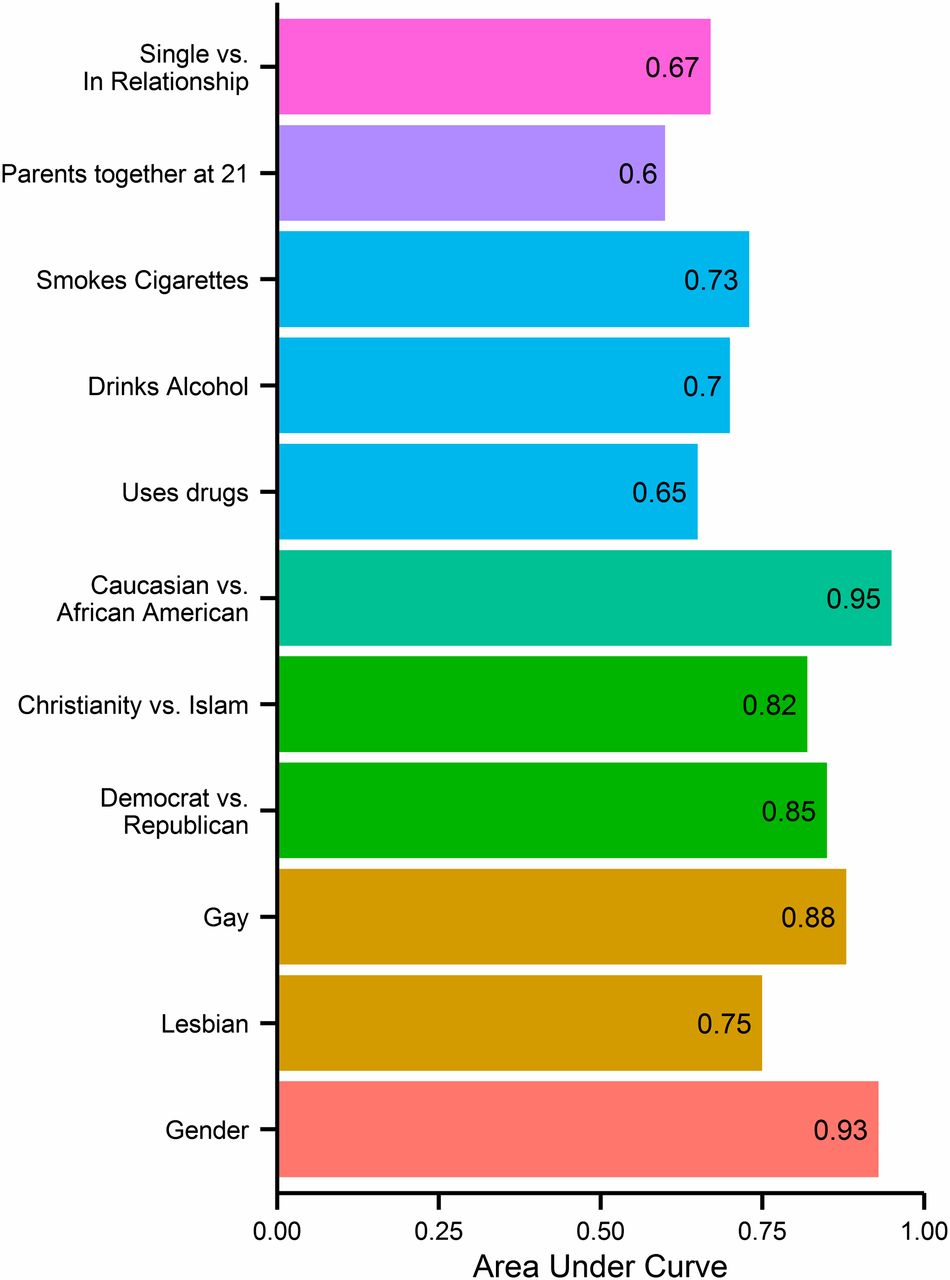
\includegraphics[scale = .6]{png/Kosinski_S1.jpg}
            \caption{Kosinski, Stillwell, \& Graepel (2013)}
        \end{figure}
    }
    \only<3>{
        \begin{figure}
            \centering
            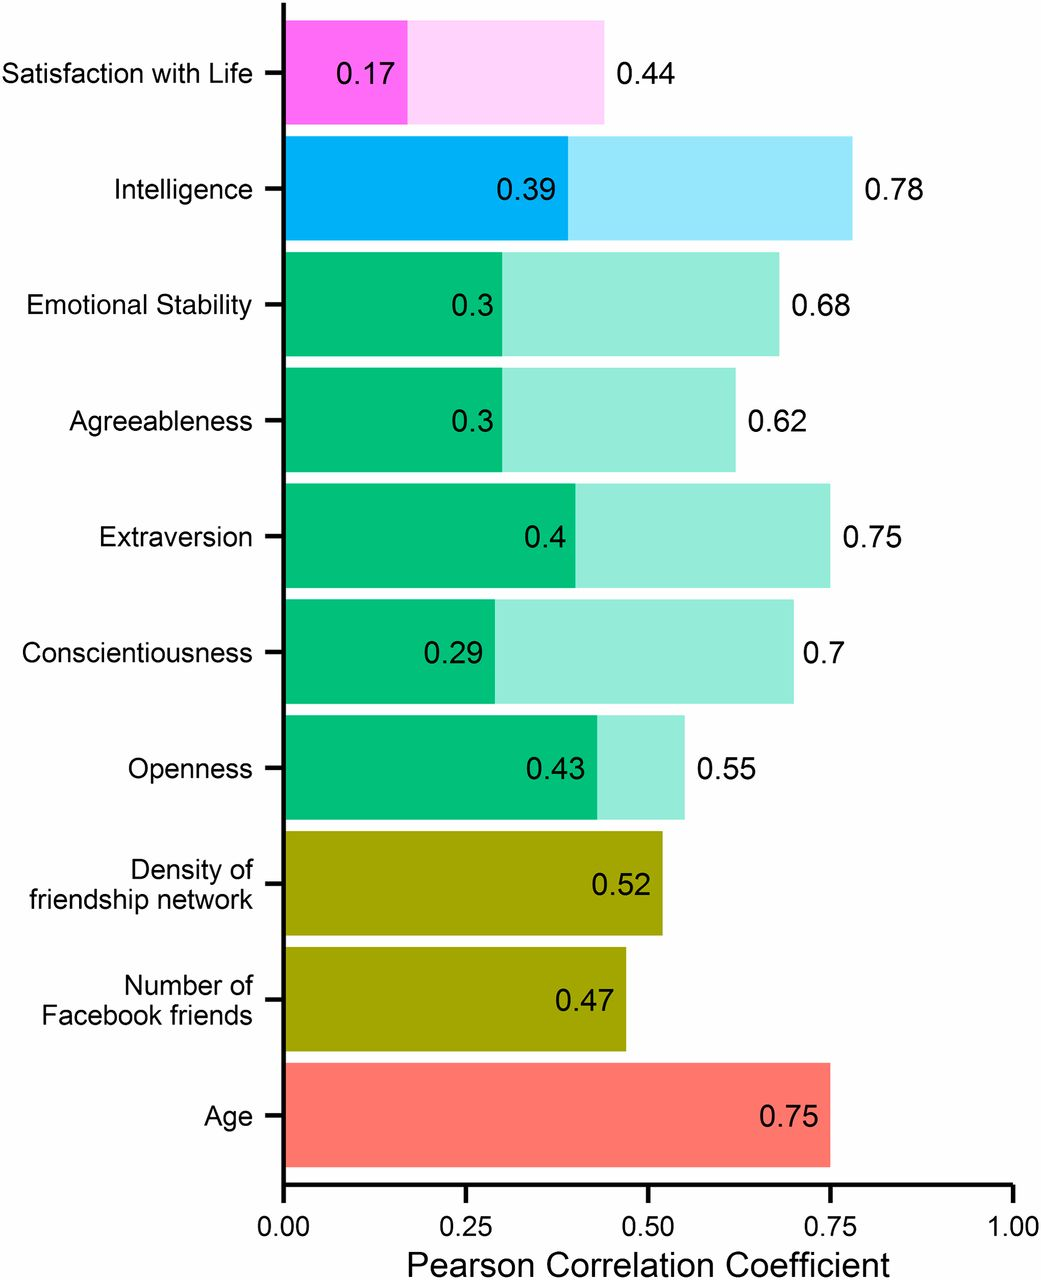
\includegraphics[scale  =.6]{png/Kosinski2_S1.jpg}
            \caption{Kosinski, Stillwell, \& Graepel (2013)}
        \end{figure}
    }
    \only<5>{
        \begin{figure}
            \centering
            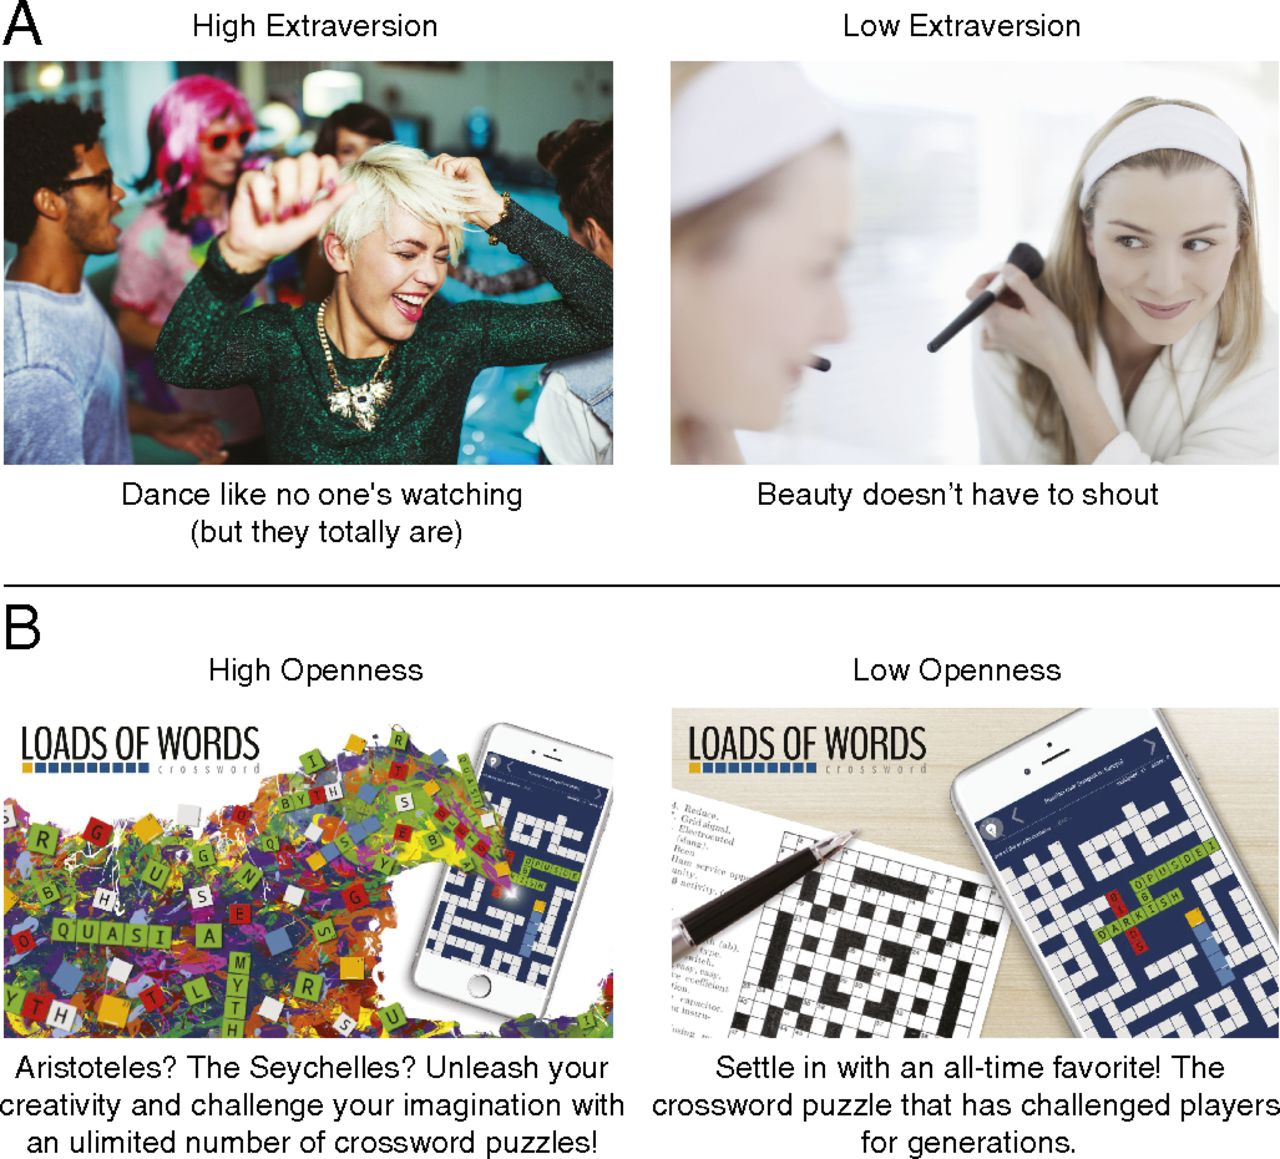
\includegraphics[scale = .6]{png/Kosinski_S2.jpg}
            \caption{Matz et al., (2017)}
        \end{figure}
    }
    \only<6>{
        \begin{figure}
            \centering
            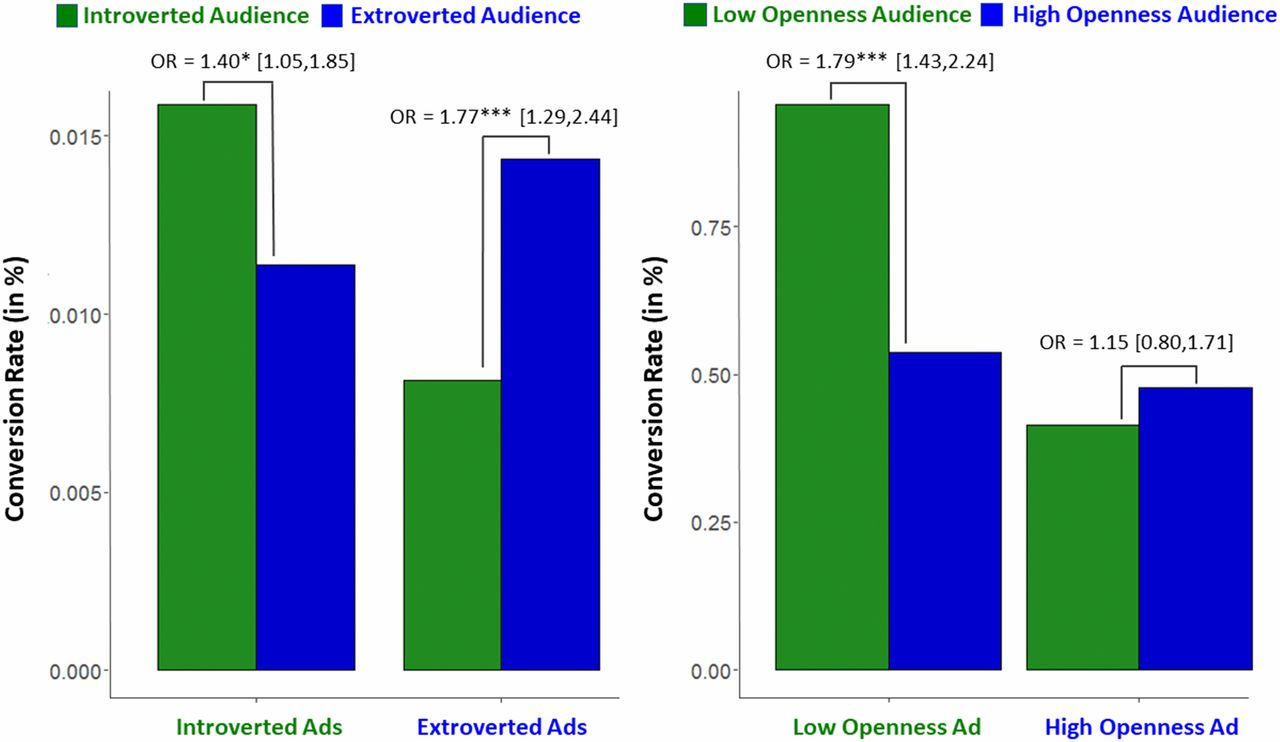
\includegraphics[scale = .8]{png/Kosinski2_S2.jpg}
            \caption{Matz et al., (2017)}
        \end{figure}
    }
    \only<8>{
        \framesubtitle{Discussion}
        \begin{enumerate}
            \item Instead of testing whether ads performed better when targeted than when untargeted to the general population, Matz et al. (2017) used a weaker test in two of their three studies (Sharp, Danenberg, \& Bellman, 2018).
            \item Users are not randomly assigned to different ads, and individuals may even receive multiple ad types (Eckles, Gordon, \& Johnson, 2018).
            \item Ad platforms like Facebook optimize campaign performance by showing ads to users whom the platform expects are more likely to fulfill the campaign’s objective (Eckles, Gordon, \& Johnson, 2018).
        \end{enumerate}
    }
    \only<9>{
        \framesubtitle{Discussion}
        \begin{figure}
            \centering
            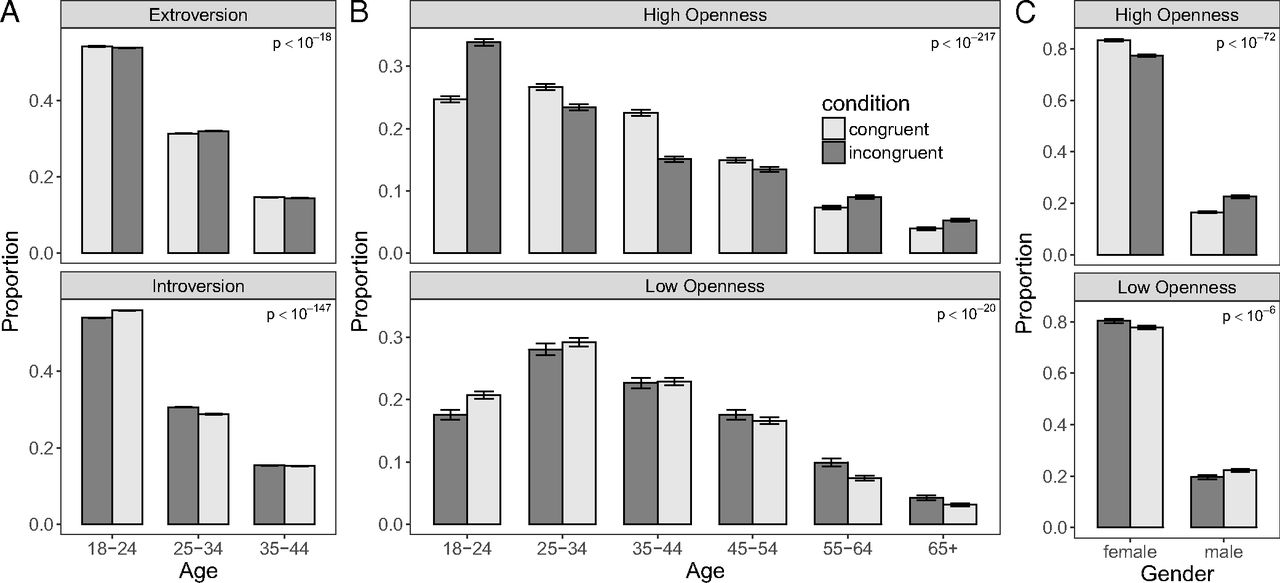
\includegraphics{png/eckels.jpeg}
            \caption{Eckles, Gordon, \& Johnson (2018)}
        \end{figure}
    }

\end{frame}

\begin{frame}
    \frametitle{Discussion}
    \only<1>{
        \begin{figure}
            \centering
            
\includegraphics[width = .9\textwidth]{zuck.jpg}
        \end{figure}
    }
    \only<2>{
        \begin{enumerate}
            \item What other exaxmples of microtargeting or psychological targeting do you know?
            \item What are the potential risks of psychological implications of psychological targeting?
            \begin{itemize}
                \item for individuals?
                \item for society?
            \end{itemize}
            \item How to prevent(?) those risks?
            \item What are the potential benefits of psychological targeting?
        \end{enumerate}
    }
\end{frame}

\begin{frame}
    \frametitle{Literature}
    \scriptsize
    \begin{enumerate}
        \item Kosinski, M., Stillwell, D., \& Graepel, T. (2013). Private traits and attributes are predictable from digital records of human behavior. Proceedings of the National Academy of Sciences, 110(15), 5802–5805. \href{https://doi.org/10.1073/pnas.1218772110}{\textcolor{blue}{https://doi.org/10.1073/pnas.1218772110}}
        \item Matz, S. C., Kosinski, M., Nave, G., \& Stillwell, D. J. (2017). Psychological targeting as an effective approach to digital mass persuasion. Proceedings of the National Academy of Sciences, 114(48), 12714–12719. \href{https://doi.org/10.1073/pnas.1710966114}{\textcolor{blue}{https://doi.org/10.1073/pnas.1710966114}}
        \item Eckles, D., Gordon, B. R., \& Johnson, G. A. (2018). Field studies of psychologically targeted ads face threats to internal validity. Proceedings of the National Academy of Sciences, 115(23), E5254–E5255. \href{https://doi.org/10.1073/pnas.1805363115}{\textcolor{blue}{https://doi.org/10.1073/pnas.1805363115}}
        \item Sharp, B., Danenberg, N., \& Bellman, S. (2018). Psychological targeting. Proceedings of the National Academy of Sciences of the United States of America, 115(34), E7890. \href{https://doi.org/10.1073/pnas.1810436115}{\textcolor{blue}{https://doi.org/10.1073/pnas.1810436115}}
    \end{enumerate}
\end{frame}


\end{document}
